% Literature review, model description and study design.
% Compile with XeLaTeX (Overleaf: Menu > Compiler > XeLaTeX), then BibTeX.
% Arial 11 pt throughout; Liberation Sans or TeX Gyre Heros are used only if
% Arial is not installed (both are metric-compatible stand-ins).
\documentclass[11pt]{article}

\usepackage[letterpaper, margin=2.2cm]{geometry}
\usepackage{fontspec}
\IfFontExistsTF{Arial}{\setmainfont{Arial}}{%
  \IfFontExistsTF{Liberation Sans}{\setmainfont{Liberation Sans}}{%
    \setmainfont{TeX Gyre Heros}}}
\usepackage[round, numbers, sort&compress]{natbib}
\usepackage[table]{xcolor}
\usepackage{booktabs, array, xltabular}
\usepackage{caption}
\usepackage{float}
\usepackage{tikz}
\usetikzlibrary{positioning, arrows.meta, calc}
\usepackage[hidelinks]{hyperref}

% Grayscale only. Captions and table text stay at the body size (11 pt).
\captionsetup{font=normalsize, labelfont=bf, justification=raggedright,
              singlelinecheck=false}
\arrayrulecolor{black!55}
\setlength{\tabcolsep}{5pt}
\renewcommand{\arraystretch}{1.25}
\setlength{\parskip}{0.5em}
\setlength{\parindent}{0pt}

\title{Food-intake detection from AIM-2 sensor signals:\\
       literature review, model description and study design}
\author{Caelan Dunlea\\University of Alabama}
\date{30 September 2026}

\begin{document}
\maketitle

\section{Literature review}
\label{sec:review}

Objective measurement of eating behaviour matters for obesity, eating
disorders and diabetes research, and self-report is known to be inaccurate
and cannot capture in-meal behaviour such as eating rate or pauses
\citep{diou2022intake}. Wearable sensors that detect chewing, bites or hand
gestures have therefore become a central approach, ranging from
classical machine learning on hand-crafted features to end-to-end deep
learning, with the aims of improving accuracy, reducing false detections
and generalising to people outside the training set \citep{bell2020scoping}.
\citet{fontana2014aim} introduced the Automatic Ingestion Monitor (AIM),
combining jaw-motion, hand-gesture and accelerometer sensors, and reported
89.8\% food-intake detection accuracy over 24 hours of free living. Its
successor, AIM-2 \citep{doulah2021aim2}, moved the sensors onto eyeglasses:
a temporalis-muscle sensor and a 3-axis accelerometer at 128\,Hz. It extracted
38 hand-crafted features per signal, selected nine by minimum-redundancy
maximum-relevance, and classified 10\,s epochs with a support vector machine,
reaching F1 0.818 under leave-one-subject-out validation on 30 participants,
as summarised in Table~\ref{tab:literature}. These feature-engineered models
work, but their performance is bounded by the features chosen by hand, and
they are sensitive to noise and to variation between people.

\begin{xltabular}{\textwidth}{@{}>{\raggedright\arraybackslash}p{30mm}
                               >{\raggedright\arraybackslash}X
                               >{\raggedright\arraybackslash}X
                               >{\raggedright\arraybackslash}X@{}}
\caption{State-of-the-art methods for food-intake and chewing detection, and
the two ECG studies whose methods transfer to this problem.}
\label{tab:literature}\\
\toprule
\rowcolor{black!8}
\textbf{References} & \textbf{Techniques} & \textbf{Goals} & \textbf{Findings} \\
\midrule
\endfirsthead
\toprule
\rowcolor{black!8}
\textbf{References} & \textbf{Techniques} & \textbf{Goals} & \textbf{Findings} \\
\midrule
\endhead
\bottomrule
\endlastfoot
\citet{doulah2021aim2} & AIM-2; hand-crafted features, mRMR selection, SVM &
  Food-intake detection with passive food-image capture &
  F1 0.818 (LOSO, 30 participants); camera triggered only during eating \\
\citet{diou2022intake} & Review: CNN on in-ear audio windows for chewing,
  smartwatch IMU for bites &
  Intake monitoring in free living &
  CNN F1 0.908 against 0.748 for an SVM; self-supervised learning comparable
  to supervised \\
\citet{kyritsis2021endtoend} & CNN + LSTM, end to end on raw wrist IMU &
  Bite and meal detection in the wild &
  Bite F1 0.923 (LOSO) \\
\citet{ghosh2022comparative} & Five deep networks (MLP, time-CNN, FCN,
  ResNet, Inception) on AIM-2 optical and accelerometer time series &
  Compare deep architectures for food-intake detection &
  ResNet best, balanced accuracy 93.47\% \\
\citet{ghosh2024integrated} & Wavelet scalogram of accelerometer, fused with
  food-image recognition &
  Reduce false positives in free living &
  Fused F1 80.77\%; fusion cuts false positives \\
\citet{stankoski2021smartwatch} & Selection of hard negative examples for
  training &
  Imbalanced data with imperfect labels &
  Person-independent F1 0.82 \\
\citet{wang2024eating} & Temporal CNN + multi-head self-attention &
  Eating speed from wrist IMU, towards free living &
  61 participants, 513\,h; eating-speed MAPE 0.110 \\
\citet{vedovelli2026recognition} & Transformer encoder and other models on
  smartwatch sensors &
  Eating-episode recognition &
  Transformer: sensitivity 0.691, specificity 0.504 (LOSO) \\
\citet{hannun2019cardiologist} & 34-layer 1D CNN on raw single-lead ECG &
  End-to-end arrhythmia classification &
  F1 0.837, above the average cardiologist (0.780) \\
\citet{ikram2025transformer} & Transformer on MIT-BIH beats &
  Five-class arrhythmia classification &
  Accuracy 97.1\%; split not at patient level \\
\end{xltabular}

\subsection{From hand-crafted features to learned representations}

To address the limits of hand-crafted features, several groups trained
networks directly on the signal. In this literature, a raw input denotes the
absence of hand-engineered features rather than of preprocessing:
z-normalisation is the only preprocessing in the convolutional time-series
baselines of \citet{wang2017strong}, and the end-to-end bite detector reviewed
by \citet{diou2022intake} receives preprocessed inertial signals.
\citet{papapanagiotou2017chewing} detected chewing with a 1D convolutional
network applied to in-ear audio windows; across window lengths of 1 to 5\,s,
the 5\,s network reached F1 0.908, against 0.748 for a support vector machine
on hand-crafted features, although such models ``require significantly
larger volumes of labeled data'' \citep{diou2022intake}. Similarly, \citet{kyritsis2021endtoend} trained a CNN feature extractor and
an LSTM jointly on raw wrist inertial data, reaching a bite-detection F1 of
0.923 under leave-one-subject-out evaluation. On AIM-2 itself,
\citet{ghosh2022comparative} compared five deep architectures on the optical
and accelerometer time series and found the residual network best, with a
balanced accuracy of 93.47\%. The same pattern holds outside eating: the
fully convolutional network of \citet{wang2017strong}, three blocks of
convolution, batch normalisation and ReLU, is a strong baseline across
time-series benchmarks.

The closest analogue to this problem is electrocardiography.
\citet{hannun2019cardiologist} classified arrhythmia with a 34-layer 1D CNN
applied end to end to raw single-lead ECG at 200\,Hz, and exceeded the
average cardiologist (F1 0.837 against 0.780). ECG and the AIM-2 signals
share a sampling rate of the same order, a quasi-periodic structure (heart
beats at about 1\,Hz, chews at 0.94--2.17\,Hz \citep{po2011chewing}) and the
need to recognise short events inside longer recordings. This motivates the
first and most important design choice in this work: the model reads the
normalised time series, not a spectrum. None of the reviewed studies
compares the two representations on the same network, so that comparison is
made directly in this work. \citet{ghosh2024integrated} took the opposite
route, converting accelerometer signals to a wavelet scalogram image. A
magnitude spectrum says which rhythms are present in a window but discards
when they occur, which is the information that separates a bite from
background motion; a scalogram keeps a time axis, but at a resolution fixed
by the transform rather than learned from the data.

\subsection{Attention and Transformers}

Attention mechanisms let a network weight the parts of its input that carry
evidence. Squeeze-and-excitation \citep{hu2018squeeze} gates feature channels
with a small learned function of their global average, at negligible cost.
Attention-based pooling \citep{ilse2018attention} treats a window as a bag
of instances and learns which instances determine its label; for eating,
the instances are time steps and a single bite may be the deciding one.
Transformers extend this to attention between all time steps.
\citet{ikram2025transformer} applied a Transformer to five-class arrhythmia
classification on MIT-BIH, reporting 97.1\% accuracy. The reported 80/20
split is of preprocessed samples rather than of patients, so the figure
measures performance on new beats from known patients, not on new
patients. In eating detection, \citet{wang2024eating} combined a temporal
CNN with multi-head self-attention to measure eating speed from wrist IMU
data on 61 participants, while \citet{vedovelli2026recognition} found that a
Transformer encoder on smartwatch data under leave-one-subject-out gave the
highest sensitivity (0.691) but a specificity of only 0.504, which is the
false-positive problem in its clearest form.

Despite their promise, Transformers carry many more parameters than the
attention layers above, and whether they help at a given data size is an
empirical question rather than a given. This work therefore uses the two
light attention mechanisms by default and treats a Transformer over the
convolutional features as a separate experiment, on the same folds.

\subsection{Supervision, augmentation and negative data}

Small annotated datasets call for more supervision per example and for more
examples per recording. Multi-task learning \citep{caruana1997multitask}
improves generalisation by training a shared representation on related
tasks; here, counting chews is the related task, since the ground truth
already contains chew annotations. This auxiliary task is specific to the
present work. Augmentation of wearable sensor data
raised accuracy from 77.54\% to 86.88\% in Parkinson's disease monitoring
\citep{um2017augmentation}; overlapping windows are the simplest form of it.
Window length itself trades resolution for context, and has a measurable
effect on recognition \citep{banos2014window}. For chewing, which ``typically
is in the range from 1 to 3\,Hz'', a 5\,s window was chosen so that ``even for
the lowest frequency of 1\,Hz, a window of 5\,s contains at least 5 periods''
\citep{diou2022intake}; the 8\,s windows used here contain at least eight.

False positives are the persistent weakness of eating detectors: many
non-eating activities produce jaw and head motion. Walking in particular has
a rhythm similar to chewing, 1 to 3\,Hz, and causes chewing classifiers ``to
yield high false-positive detections'', which accelerometer data can be used
to remove \citep{diou2022intake}. The same work notes that a detector can be
tuned ``towards higher recall or precision, or a balanced mode, based on the
needs of each use-case''. \citet{stankoski2021smartwatch}
reduced them by deliberately selecting hard negative examples for training,
and \citet{ghosh2024integrated} by fusing the sensor classifier with food-image
recognition. Finally, evaluation practice varies widely across the field
\citep{bell2020scoping}. \citet{saeb2017need} showed that record-wise
cross-validation, where windows from one person appear in both training and
test sets, can massively overestimate accuracy, and that subject-wise
validation is the one that matches the use case. The leave-one-subject-out
protocol used by \citet{doulah2021aim2} and \citet{diou2022intake} is adopted
here for the same reason.

\subsection{Contribution of this work}

\begin{itemize}
  \item A compact convolutional model with channel attention, temporal
        attention pooling and an auxiliary chew-count head, reading the
        normalised AIM-2 optical and accelerometer signals directly from the
        ETS database: 61 annotated sessions from 43 participants, evaluated
        at the participant level.
  \item A direct comparison of time-series and spectral input on the same
        network, which none of the reviewed studies reports. The time
        series reaches F1 0.858 against 0.796 and reduces false alarms from
        81 to 32 per hour of non-eating.
  \item A controlled ablation of each design decision, one at a time on
        identical participant-level folds, separating the components that
        carry the performance from those that do not.
  \item Negative results reported with their mechanism: temporal median
        smoothing and context windows without a target marker both lower
        F1, because meals at 8\,s resolution are punctuated rather than
        contiguous.
  \item A measured check of sensor-annotation alignment on every session,
        replacing an assumed correction with a verified one.
\end{itemize}

Despite the progress in deep learning for intake monitoring, several
challenges persist: limited annotated data, variation between participants
in sensor fit and chewing style, false positives from non-eating jaw and head
motion, and inconsistent evaluation that makes published results hard to
compare. Addressing these requires models that generalise to people they
have not seen, evaluated in the way they would be used.

\section{Model description}
\label{sec:model}

The model is a compact one-dimensional convolutional network that reads the
raw AIM-2 sensor signals and outputs the probability that an 8\,s window
contains eating (Figure~\ref{fig:architecture}). It has four parts. A
convolutional feature extractor learns its own filters from the time series
instead of receiving hand-crafted features or a spectrum. A squeeze-and-excitation
gate reweights the learned feature channels in each window. An attention
pooling layer weights the time steps that carry the evidence. Finally, the
output has two heads: one classifies eating, and one counts chews and is used
only during training. The network has 47,282 parameters at inference
(Table~\ref{tab:layers}). Table~\ref{tab:model} lists every design decision
with its reason and the literature it rests on.

\begin{figure}[H]
\centering
% Model architecture, top to bottom. Grayscale only; font inherited from the
% document (Arial 11). Drawn at final size - never scale it, or the text stops
% being 11 pt. Used by literature_review.tex and figure_architecture.tex.
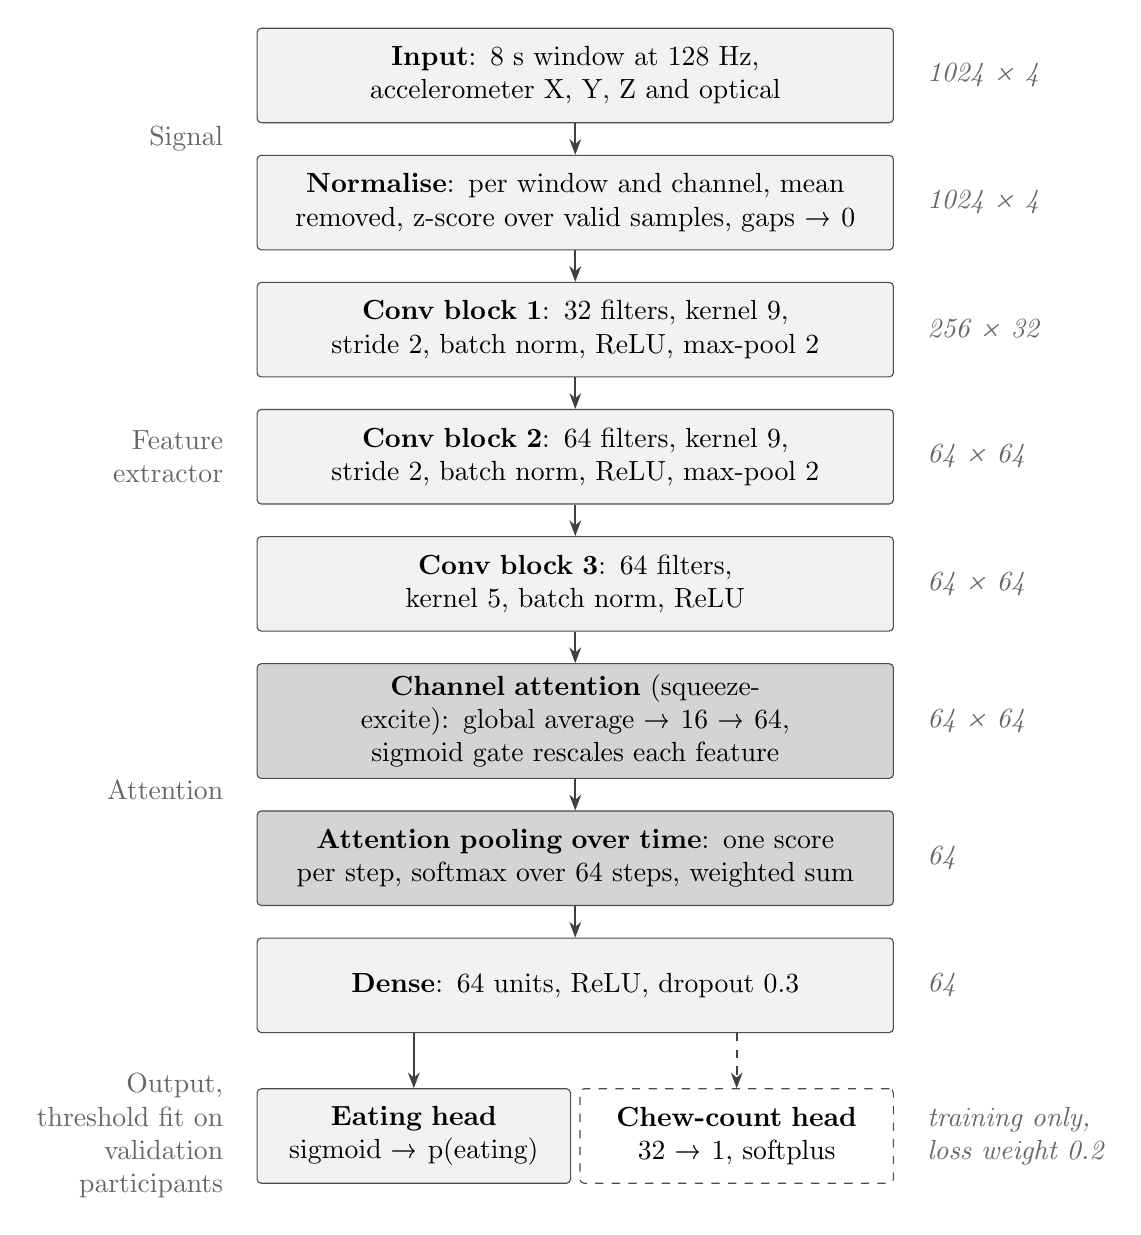
\begin{tikzpicture}[
    box/.style   = {draw=black!70, fill=black!5, rounded corners=1.5pt,
                    align=center, inner sep=4pt, text width=78mm, execute at begin node={\hyphenpenalty=10000},
                    minimum height=12mm},
    key/.style   = {box, fill=black!17},
    head/.style  = {box, text width=37mm},
    flow/.style  = {-{Stealth[length=2mm]}, draw=black!75, line width=0.6pt},
    dims/.style = {text=black!60, font=\itshape, anchor=west},
    stage/.style = {text=black!60, anchor=east, align=right, execute at begin node={\hyphenpenalty=10000}},
    node distance = 4mm,
  ]
  \node[box] (in)
      {\textbf{Input}: 8 s window at 128 Hz, accelerometer X, Y, Z and optical};
  \node[box, below=of in] (norm)
      {\textbf{Normalise}: per window and channel, mean removed, z-score over valid samples, gaps → 0};
  \node[box, below=of norm] (c1)
      {\textbf{Conv block 1}: 32 filters, kernel 9, stride 2, batch norm, ReLU, max-pool 2};
  \node[box, below=of c1] (c2)
      {\textbf{Conv block 2}: 64 filters, kernel 9, stride 2, batch norm, ReLU, max-pool 2};
  \node[box, below=of c2] (c3)
      {\textbf{Conv block 3}: 64 filters, kernel 5, batch norm, ReLU};
  \node[key, below=of c3] (se)
      {\textbf{Channel attention} (squeeze-excite): global average → 16 → 64, sigmoid gate rescales each feature};
  \node[key, below=of se] (ap)
      {\textbf{Attention pooling over time}: one score per step, softmax over 64 steps, weighted sum};
  \node[box, below=of ap] (fc)
      {\textbf{Dense}: 64 units, ReLU, dropout 0.3};
  \node[head, below=7mm of fc.south west, anchor=north west] (food)
      {\textbf{Eating head}\\sigmoid → p(eating)};
  \node[head, dashed, fill=white, below=7mm of fc.south east, anchor=north east] (chew)
      {\textbf{Chew-count head}\\32 → 1, softplus};

  \foreach \a/\b in {in/norm, norm/c1, c1/c2, c2/c3, c3/se, se/ap, ap/fc}
    \draw[flow] (\a) -- (\b);
  \draw[flow] (fc.south -| food.north) -- (food.north);
  \draw[flow, dashed] (fc.south -| chew.north) -- (chew.north);

  % output shapes, right of each block
  \foreach \n/\s in {in/1024 × 4, norm/1024 × 4, c1/256 × 32, c2/64 × 64,
                     c3/64 × 64, se/64 × 64, ap/64, fc/64}
    \node[dims] at ([xshift=3mm]\n.east) {\s};
  \node[dims, align=left] at ([xshift=3mm]chew.east) {training only,\\loss weight 0.2};

  % stages, left of the column
  \node[stage] at ([xshift=-3mm]$(in.west)!0.5!(norm.west)$) {Signal};
  \node[stage] at ([xshift=-3mm]c2.west) {Feature\\extractor};
  \node[stage] at ([xshift=-3mm]$(se.west)!0.5!(ap.west)$) {Attention};
  \node[stage] at ([xshift=-3mm]food.west) {Output,\\threshold fit on\\validation\\participants};
\end{tikzpicture}

\caption{Model architecture. Shaded blocks are the two attention mechanisms.
The dashed chew-count head is trained jointly and discarded at inference.
Output shapes are time steps × features.}
\label{fig:architecture}
\end{figure}

% Layer-by-layer dimensions and parameter counts (inference model plus the
% training-only chew head). Counts computed from the layer definitions in
% scripts/train_food_intake.build_attention_cnn.
\begin{table}[H]
\centering
\caption{Layer dimensions. An 8\,s window at 128\,Hz is 1024 samples; each of
the 64 output time steps covers about 0.9\,s of signal at 125\,ms spacing.}
\label{tab:layers}
\begin{tabular}{@{}llrr@{}}
\toprule
\rowcolor{black!8}
\textbf{Layer} & \textbf{Configuration} & \textbf{Output} & \textbf{Parameters} \\
\midrule
Input            & Acc X, Y, Z, Optical            & 1024 × 4  & -- \\
Conv block 1     & 32 × \textit{k}9, stride 2, BN, max-pool 2 & 256 × 32  & 1,312 \\
Conv block 2     & 64 × \textit{k}9, stride 2, BN, max-pool 2 & 64 × 64   & 18,752 \\
Conv block 3     & 64 × \textit{k}5, BN                       & 64 × 64   & 20,800 \\
Channel attention & 64 → 16 → 64, sigmoid          & 64 × 64   & 2,128 \\
Attention pooling & 1 × 1 conv, softmax over time  & 64        & 65 \\
Dense            & 64, ReLU, dropout 0.3           & 64        & 4,160 \\
Eating head      & 1, sigmoid                      & 1         & 65 \\
\midrule
\multicolumn{3}{@{}l}{\textit{Total at inference}}               & \textit{47,282} \\
Chew-count head  & 32 → 1, softplus (training only) & 1        & 2,113 \\
\bottomrule
\end{tabular}
\end{table}


% Complete model description, one row per design decision.
% Style follows the 9/22 lab-meeting table: #, component, choice, why - plus
% the literature each decision rests on.
\begin{xltabular}{\textwidth}{@{}>{\raggedright\arraybackslash}p{5mm}
                               >{\raggedright\arraybackslash}p{24mm}
                               >{\raggedright\arraybackslash}X
                               >{\raggedright\arraybackslash}X
                               >{\raggedright\arraybackslash}p{24mm}@{}}
\caption{Complete description of the food-intake detection model. Every design
decision, the reason for it, and the literature it is grounded in.}
\label{tab:model}\\
\toprule
\rowcolor{black!8}
\textbf{\#} & \textbf{Component} & \textbf{Design} & \textbf{Why} & \textbf{Literature} \\
\midrule
\endfirsthead
\toprule
\rowcolor{black!8}
\textbf{\#} & \textbf{Component} & \textbf{Design} & \textbf{Why} & \textbf{Literature} \\
\midrule
\endhead
\midrule
\multicolumn{5}{r@{}}{\textit{continued on next page}} \\
\endfoot
\bottomrule
\endlastfoot

\multicolumn{5}{@{}l}{\textit{Data}} \\
1 & Sensor & AIM-2 eyeglass sensor: 3-axis accelerometer and optical temporalis-muscle sensor, 128\,Hz, stored as 8\,s packets in the ETS database & Chewing moves the temporalis muscle and the head; both channels carry it, with different artefacts. The original AIM-2 used a flex sensor where this one has the optical sensor & \citet{doulah2021aim2, ghosh2022comparative} \\
2 & Labels & Eating = bout OR bite annotation at 10\,Hz. Window is eating if more than half its annotated samples are eating. Unrecorded time (−1) is dropped, never treated as non-eating & Treating unannotated time as negative would bury the real labels and invent easy negatives & (this work) \\
3 & Alignment & No time shift. Sensor/annotation lag measured by cross-correlating the optical chewing envelope with the labels: median +0.10\,s, all within 0.2\,s on the 20 sessions measured first (to be repeated on all 61) & A correction must be measured, not assumed; a residual lag of one packet would corrupt every label edge & (this work) \\
4 & Window & 8\,s (1024 samples), non-overlapping at evaluation & Chewing lies at 1--3\,Hz; a 5\,s window was chosen for chewing detection so that it holds at least five chews, and AIM-2 used 10\,s epochs. An 8\,s window holds at least eight chews and matches the packet size. Lengths of 2--16\,s are also evaluated & \citet{diou2022intake, doulah2021aim2, po2011chewing} \\

\multicolumn{5}{@{}l}{\textit{Input}} \\
5 & Representation & Normalised time series, 1024 samples × 4 channels; no spectrum and no hand-crafted features & In the reviewed studies, features learned from the signal outperformed hand-engineered ones. None compares time-series and spectral input on the same network; that comparison is made here (61 sessions, 5-fold): F1 0.858 against 0.796, and 32 against 81 false alarms per hour of non-eating & \citet{ghosh2022comparative, kyritsis2021endtoend, diou2022intake}; this work \\
6 & Normalisation & Per window, per channel: mean removed, z-scored over valid samples only; missing samples set to 0 after scaling & Optical baseline varies by participant and fit on the face; DC level is not information about chewing. A literal −1 against counts near 3000 injects a step at every gap. z-normalisation is likewise the only preprocessing in the standard convolutional time-series baselines & \citet{wang2017strong} \\

\multicolumn{5}{@{}l}{\textit{Network}} \\
7 & Convolutional trunk & Three 1D conv blocks: 32@\textit{k}9/s2, 64@\textit{k}9/s2, 64@\textit{k}5, each with batch norm and ReLU, max-pool 2 after the first two. Output 64 time steps × 64 features & Learns its own filters from the signal. For chewing detection, a CNN reached F1 0.908 against 0.748 for an SVM on hand-crafted features. Each output step covers about 0.9\,s of signal (one chew cycle) at 125\,ms spacing & \citet{wang2017strong, ghosh2022comparative, diou2022intake, hannun2019cardiologist} \\
8 & Channel attention & Squeeze-and-excitation: global average → dense 16 (ReLU) → dense 64 (sigmoid) → rescale each feature channel & Walking at 1--3\,Hz resembles chewing and produces false positives in chewing detectors; the accelerometer is what separates the two. The gate reweights optical against motion channels in every window at negligible cost & \citet{hu2018squeeze, diou2022intake} \\
9 & Temporal pooling & Attention pooling: one score per time step (1 × 1 conv), softmax over the 64 steps, weighted sum & Global averaging dilutes a 1--2\,s bite across 8\,s. Attention weights the informative steps, as in multiple-instance learning & \citet{ilse2018attention} \\
10 & Classifier & Dense 64 (ReLU), dropout 0.3, sigmoid output & Small head; about 47\,k parameters in total at inference & -- \\
11 & Auxiliary head & Chew-count regression (dense 32 → 1, softplus), target scaled by its 99th percentile. Used in training only & Deep models require large volumes of labelled data, and one label bit per window is thin supervision. The chew-count task is specific to this work; the principle is multi-task learning & \citet{caruana1997multitask, diou2022intake} \\

\multicolumn{5}{@{}l}{\textit{Training}} \\
12 & Loss & Binary cross-entropy (weight 1.0) + chew MSE (weight 0.2); class-balanced sample weights computed per fold & Auxiliary loss is a regulariser, not the objective. Eating fraction ranges 0--86\% by session, so the rare class changes with the fold & \citet{caruana1997multitask} \\
13 & Augmentation & 50\% overlapping windows (4\,s hop) at training time only & Roughly doubles the training windows at no collection cost; evaluation stays on the non-overlapping grid so no second is scored twice & \citet{um2017augmentation} \\
14 & Optimisation & Adam, learning rate 0.0003, batch 64, up to 80 epochs, early stopping (patience 12) and learning-rate halving on validation ROC AUC & At 0.001 the validation optimum fell at the first epoch in most folds; the lower rate moves it later. Validation participants are held out from training, never random windows & -- \\

\multicolumn{5}{@{}l}{\textit{Evaluation}} \\
15 & Validation & Leave-one-subject-out: 43 folds, each holding out one participant with all of their sessions. Inner validation on further held-out participants & Windows of one meal are near-duplicates; any split below participant level leaks and overstates performance. Leave-one-subject-out is the protocol of the AIM-2 and smartwatch intake studies & \citet{doulah2021aim2, kyritsis2021endtoend, diou2022intake, saeb2017need} \\
16 & Threshold & Chosen on the inner validation participants, never on the test participant: at the centre of the F1 plateau by default, or as the highest recall within a false-alarm budget per hour & The F1 curve is flat near its peak, so its exact argmax on few participants is noise. A detector can be tuned towards recall or precision according to the use case; in free living, false alarms carry the higher cost & \citet{diou2022intake} \\
17 & Post-processing & None. Median smoothing over 3 windows was tested and rejected (F1 −0.079) & Meals are punctuated by pauses; at 8\,s the label genuinely switches, and smoothing erases short real bouts & (this work) \\
18 & Metrics & F1 and balanced accuracy lead; accuracy, precision, recall and false alarms per hour of non-eating reported alongside, pooled over all held-out windows and per participant & Class balance differs by participant; accuracy alone rewards predicting the majority class. False alarms per hour expresses the free-living failure mode directly & \citet{bell2020scoping} \\
\end{xltabular}


\subsection{Dataset and current performance}

The dataset is 61 annotated eating sessions (breakfast, lunch, dinner and
snack) from 43 participants, 2 to 55 minutes each: 24.2 hours of annotated
recording, of which 9.6 hours is eating. The eating fraction ranges from 0\%
to 86\% by session. Validation is leave-one-subject-out: 43 folds, each
holding out one participant with all of their sessions.

In a preliminary participant-level 5-fold cross-validation, pooled over all
10,891 held-out non-overlapping windows, the model reaches F1 0.858,
accuracy 0.891, balanced accuracy 0.881, precision 0.884 and recall 0.834,
with 32 false alarms per hour of non-eating. Per-participant F1 has mean
0.835 (standard deviation 0.136, median 0.878); the spread between people is
the honest measure of how the model generalises to someone new, and it is
larger than any difference between design choices seen so far.
Leave-one-subject-out results will replace these figures.

\section{Proposed study design}
\label{sec:plan}

The literature review points to one gap more than any
other: food-intake detectors from wearable chewing sensors are usually
reported as a single architecture with a single number, and the design
decisions behind them are rarely isolated. The ablation in
Table~\ref{tab:ablation} already shows that those decisions are not equally
important, since the input representation accounts for most of the
performance and the attention components cannot be separated from noise.
The proposed study makes that the question rather than a side result: which
design dimensions matter for deep food-intake detection from a chewing
sensor, measured one at a time under leave-one-subject-out validation.

\begin{table}[H]
\centering
\caption{Preliminary ablation: the model with one component removed or
added. The first 20 annotated sessions, participant-level 4-fold
cross-validation, same folds for every row. Fold-to-fold spread in F1 was
about 0.048, so effects smaller than that are not distinguishable from
noise. To be repeated on all 61 sessions.}
\label{tab:ablation}
\begin{tabular}{@{}lrrrl@{}}
\toprule
\rowcolor{black!8}
\textbf{Variant} & \textbf{F1} & \textbf{Change} & \textbf{Precision} & \textbf{Verdict} \\
\midrule
Full model                             & 0.854 & --     & 0.876 & -- \\
FFT magnitude input instead of time series & 0.767 & −0.087 & 0.696 & Hurts \\
No overlapping training windows        & 0.829 & −0.025 & 0.834 & Possibly hurts \\
No attention (global average pooling)  & 0.847 & −0.007 & 0.857 & Within noise \\
No chew-count head                     & 0.849 & −0.006 & 0.857 & Within noise \\
Add median smoothing (3 windows)       & 0.775 & −0.079 & 0.765 & Hurts \\
Add 8\,s context each side, no marker  & 0.775 & −0.080 & 0.683 & Hurts \\
\bottomrule
\end{tabular}
\end{table}

\subsection{Protocol, fixed for every experiment}

\begin{itemize}
  \item \textbf{Leave-one-subject-out validation} on all 43 participants
        (43 folds, each holding out every session of one participant),
        following \citet{saeb2017need}. At about a minute per fold this is
        computationally feasible, and it is the closest approximation of
        the use case: a participant the model has never seen. Five-fold
        runs are used only to explore.
  \item \textbf{Paired comparison per participant.} Each variant is scored
        on the same held-out participants as the reference model, so the
        difference can be tested per participant (Wilcoxon signed-rank)
        rather than read against the spread of fold means.
  \item \textbf{Three seeds per configuration}, reported as mean and range,
        so initialisation noise is not mistaken for an effect.
  \item \textbf{False positives per hour of non-eating} reported alongside
        F1, because that is the failure mode that matters in free-living use
        and the one negative data (below) is meant to fix.
\end{itemize}

\subsection{Dimensions to explore}

\begin{xltabular}{\textwidth}{@{}>{\raggedright\arraybackslash}p{27mm}
                               >{\raggedright\arraybackslash}X
                               >{\raggedright\arraybackslash}X
                               >{\raggedright\arraybackslash}p{26mm}@{}}
\caption{Planned experiments. Each changes one dimension of the model in
the model and holds everything else fixed.}
\label{tab:plan}\\
\toprule
\rowcolor{black!8}
\textbf{Dimension} & \textbf{Levels} & \textbf{Question} & \textbf{Grounding} \\
\midrule
\endfirsthead
\toprule
\rowcolor{black!8}
\textbf{Dimension} & \textbf{Levels} & \textbf{Question} & \textbf{Grounding} \\
\midrule
\endhead
\bottomrule
\endlastfoot
Published architectures & FCN, ResNet and Inception as compared by
  \citet{ghosh2022comparative}, trained on the same folds &
  Where does this model stand against the closest prior work on AIM-2, under
  an identical protocol? &
  \citet{ghosh2022comparative, wang2017strong} \\
Input representation & Time series, FFT magnitude, wavelet scalogram &
  Does keeping temporal structure explain the gain, and does a
  time-frequency image recover it? &
  \citet{ghosh2024integrated, hannun2019cardiologist} \\
Sampling rate & 128, 64, 32, 16\,Hz &
  How much of the signal is needed? Chewing lies below about 2.2\,Hz, so
  32\,Hz still leaves a Nyquist margin of seven times. &
  \citet{po2011chewing} \\
Window length & 2, 4, 8, 16\,s &
  Resolution against context: shorter windows localise bites, longer
  windows contain more chew cycles. &
  \citet{banos2014window} \\
Context & None; 8\,s each side with a target-window marker channel &
  Can surrounding signal help without the model answering "is there eating
  anywhere nearby?" &
  (this work) \\
Chew-head weight & 0, 0.1, 0.2, 0.5, 1.0 &
  How strongly should counting chews shape the features, and does it help
  participants with weak optical signal? &
  \citet{caruana1997multitask} \\
Temporal model & Attention pooling; small Transformer encoder over the 64
  convolutional time steps &
  Does self-attention between time steps add to a convolutional front end
  at this data size? &
  \citet{ikram2025transformer, zerveas2021transformer, zeng2023transformers} \\
Self-supervised pre-training & None; convolutional trunk pre-trained on
  unannotated AIM-2 recordings in ETS &
  Can the unannotated sensor data, most of what the database holds, stand
  in for labels the study does not have? &
  \citet{diou2022intake} \\
Negative data & Annotated sessions only; plus non-eating recordings from
  other ETS studies &
  Do additional negative participants reduce false positives without
  costing recall? &
  \citet{bell2020scoping, ghosh2024integrated} \\
\end{xltabular}

The published-architecture row comes first: it is the comparison a reviewer
will ask for, and it replaces comparisons with the lab's earlier model. The
representation, sampling-rate and window rows are cheap and answer the
questions raised at the 9/23 lab meeting directly. The Transformer row is the one most likely to be
asked about by reviewers, and the one most at risk of overfitting on a
dataset this size; with 24 hours of annotated data it is now worth running, and
should be reported whether it helps or not. Negative
data is expected to have the largest practical effect, since false
positives are the model's main weakness, and is the natural joint
experiment with the lab.


\bibliographystyle{unsrtnat}
\bibliography{refs}

\end{document}
